%%%%%%%%%%%%%%%%%%%%%%%%%%%%%%%%%%%%%%%%%%%%%%%%%%%%%%%%%%
%%
%% MARK: Title & Data
%%
%%%%%%%%%%%%%%%%%%%%%%%%%%%%%%%%%%%%%%%%%%%%%%%%%%%%%%%%%%

\chapter*{\S B15. $p$-Forms on Half-Spaces}
\setcounter{footnote}{0}

%%%%%%%%%%%%%%%%%%%%%%%%%%%%%%%%%%%%%%%%%%%%%%%%%%%%%%%%%%
%%
%% MARK: Abstract
%%
%%%%%%%%%%%%%%%%%%%%%%%%%%%%%%%%%%%%%%%%%%%%%%%%%%%%%%%%%%

\begin{abstract}
  We shall see that every differential $p$-form on the half-space $H^n = [0,\infty[ \,\times\, \RR^{n-1}$ is the restriction of a smooth $p$-form on $\RR^n$.
\end{abstract}

%%%%%%%%%%%%%%%%%%%%%%%%%%%%%%%%%%%%%%%%%%%%%%%%%%%%%%%%%%
%%
%% MARK: Content
%%
%%%%%%%%%%%%%%%%%%%%%%%%%%%%%%%%%%%%%%%%%%%%%%%%%%%%%%%%%%

This note is a natural development of the previous ``$1$-Forms on Half-Spaces''.

\begin{Article}{Differential $p$-forms on half-spaces.}{}
  Let $H^n = [0,\infty[ \,\times\, \RR^{n-1}$ be the half $n$-space,
  equipped with the subset diffeology.
  Let $\omega \in \DForms^p(H^n)$ be a differential $p$-form on $H^n$.
  Then,
  there exists a smooth $p$-form $\bar\omega$ defined on some neighborhood of $H^n \subset \RR^n$ such that $\omega = \bar\omega \restriction H^n$.
\end{Article}

\begin{proof}
  Since $\mathring{H}{}^n = ]0,\infty[ \,\times\, \RR^{n-1} \subset H^n = [0,\infty[ \,\times\, \RR^{n-1}$ inherits the usual smooth diffeology,
  \begin{align*}
    \omega \restriction \mathring{H}{}^n & = \sum_{\substack{1<j<\dots<k}} a_{1j\dots k}(x,y) \, dx \wedge dy_j \wedge \dots \wedge dy_k \\
    & + \sum_{\substack{i<j<\cdots<k}} b_{ij\dots k}(x,y) \, dy_i \wedge dy_j \wedge \dots \wedge dy_k,
  \end{align*}
  where $(x,y) \in \mathring{H}{}^n$ and $a_{1j\dots k}, b_{ij\dots k} \in \Cinfty(\mathring{H}{}^n,\RR)$.
  
  Now,
  let
  $$
    \Sq_1 : (t,y) \mapsto (t^2,y),
  $$
  then
  %
  \begin{align*}
    \Sq_1^*(\omega) & = \omega((t,y) \mapsto (t^2,y)) \\
    & = \sum_{\substack{1<j<\dots<k}} A_{1j\dots k}(t,y) \, dt \wedge dy_j \wedge \dots \wedge dy_k \\
    & + \sum_{\substack{i<j<\dots<k}} B_{ij\dots k}(t,y) \, dy_i \wedge dy_j \wedge \dots \wedge dy_k,
  \end{align*}
  %
  with $A_{1j\dots k}, B_{ij\dots k} \in \Cinfty(\RR^n,\RR)$.
  For all $t \neq 0$,
  $$
    A_{1j\dots k}(t,y) = 2t \, a_{1j\dots k}(t^2,y) \quad \text{and} \quad B_{ij\dots k}(t,y) = b_{ij\dots k}(t^2,y).
  $$
  
  Next,
  $\Sq_1^*(\omega)$ is invariant under $\epsilon : (t,y) \mapsto (-t,y)$,
  thus
  %
  \begin{align*}
    \Sq_1^*(\omega) & = \epsilon^*(\Sq_1^*(\omega)) \\
    & = \sum_{\substack{1<j<\dots<k}} A_{1j\dots k}(-t,y) \, (-dt \wedge dy_j \wedge \dots \wedge dy_k) \\
    & + \sum_{\substack{i<j<\dots<k}} B_{ij\dots k}(-t,y) \, dy_i \wedge dy_j \wedge \dots \wedge dy_k.
  \end{align*}
  %
  Hence,
  $-A_{1j\dots k}(-t,y) = A_{1j\dots k}(t,y)$ and $B_{ij\dots k}(t,y) = B_{ij\dots k}(-t,y)$.
  In particular,
  $A_{1j\dots k}(0,y) = 0$.
  Therefore,
  there exists a smooth function $\underline{A}_{1j\dots k} \in \Cinfty(\RR^n,\RR)$ such that $A_{1j\dots k}(t,y) = 2t \,\underline{A}_{1j\dots k}(t,y)$,
  for all $t \in \RR$.
  Thus,
  for all $t \neq 0$,
  $a_{1j\dots k}(t^2,y) = \underline{A}_{1j\dots k}(t,y)$.
  Now, $\underline{A}_{1j\dots k}$ is even in $t$,
  as are the $B_{ij\dots k}$.
  We can then apply the Hassler Whitney theorem \cite[Theorem 1 and final remark]{Whi43},
  stated as follows:
  
  \uline{Theorem. (Whitney)} {\itshape If a smooth function $f(t,x)$ is even in $t$,
  $f(t,x) = f(-t,x)$,
  then there exists a smooth function $g(t,x)$ such that $f(t,x) = g(t^2,x)$.}
  
  Hence,
  there exist smooth functions $\underline{a}_{1j\dots k}(x,y)$ and $\underline{b}_{ij\dots k}(x,y)$,
  such that $\underline{A}_{1j\dots k}(t,y) = \underline{a}_{1j\dots k}(t^2,y)$ and $B_{ij\dots k}(t,y) = \underline{b}_{ij\dots k}(t^2,y)$.
  Then,
  for all $t > 0$,
  $a_{1j\dots k}(t,y) = \underline{a}_{1j\dots k}(t,y)$ and $b_{ij\dots k}(t,y) = \underline{b}_{ij\dots k}(t,y)$.
  
  Let us then define $\bar\omega$ on $\RR^n$:
  %
  \begin{align*}
    \bar\omega & = \sum_{\substack{1<j<\dots<k}} \underline{a}_{1j\dots k}(x,y) \, dx \wedge dy_j \wedge \dots \wedge dy_k \\
    & + \sum_{\substack{i<j<\dots<k}} \underline{b}_{ij\dots k}(x,y) \, dy_i \wedge dy_j \wedge \dots \wedge dy_k.
  \end{align*}
  %
  The form $\bar\omega$ is a smooth $p$-form defined on an open neighborhood of $H^n$,
  and $\omega \restriction \mathring{H}{}^n = \bar\omega \restriction \mathring{H}{}^n$.
  %
  Let us now prove that $\omega$ and $\bar\omega$ coincide on the whole $H^n$.
  Since $\omega$ and $\bar\omega \restriction H^n$ are two differential $p$-forms on $H^n$,
  it is sufficient to check that they take the same value on every smooth $p$-path.
  
  Let $\sigma$ be any $p$-path in $H^n$.
  Let $\cO = \sigma^{-1}(\mathring{H}{}^n)$,
  which is open in $\RR^p$,
  and on this open subset $\bar\omega(\sigma) = \omega(\sigma)$.
  Hence,
  by continuity $\bar\omega(\sigma) = \omega(\sigma)$ on the closure $\overline \cO$ of $\cO$
  (since $\bar\omega(\sigma)$ and $\omega(\sigma)$ are smooth).
  
  On the open subset $\RR^p - \overline{\cO}$,
  $\sigma$ takes its values in $\partial H^n = \{0\} \times \RR^{n-1}$;
  $\bar\sigma = \sigma \restriction (\RR^p - \overline{\cO})$ is a plot of the boundary $\partial H^n$.
  Let $i: \RR^{n-1} \to \partial H^n$,
  $i(y) = (0,y)$.
  Then,
  $i^*(\omega)$ and $i^*(\bar\omega)$ are both $p$-forms on $\RR^{n-1}$.
  Let us prove that they coincide.
  On the one hand,
  $$
    i^*(\bar\omega) = \sum_{\substack{i<j<\dots<k}} \underline{b}_{ij\dots k}(0,y) \, dy_i \wedge dy_j \wedge \dots \wedge dy_k.
  $$
  On the other hand,
  note that
  $$
    i = \Sq_1 \circ i : y \mapsto (0,y) \mapsto (0^2,y).
  $$
  Thus,
  $i^*(\omega) = i^*(\Sq_1^*(\omega))$ and then
  $$
    i^*(\omega)_y(\delta_1 y, \dots, \delta_{p-1} y) = \Sq_1^*(\omega)_{(0,y)}(0, \delta_1 y, \dots, \delta_{p-1} y).
  $$
  Hence,
  %
  \begin{align*}
    \Sq_1^*(\omega) & = \sum_{\substack{i<j<\dots<k}} B_{ij\dots k}(0,y) \, dy_i \wedge dy_j \wedge \dots \wedge dy_k \\
    & = \sum_{\substack{i<j<\dots<k}} \underline{b}_{ij\dots k}(0,y) \, dy_i \wedge dy_j \wedge \dots \wedge dy_k,
  \end{align*}
  %
  since $A_{1j\dots k}(0,y) = 0$ and $B_{ij\dots k}(t,y) = \underline{b}_{ij\dots k}(t^2,y)$.
  
  Hence $\omega$ and $\bar\omega$ coincide on $\partial H^n$, and therefore $\bar\omega(\sigma)$ and $\omega(\sigma)$ coincide everywhere.
  %
  Consequently,
  since $\bar\omega$ and $\omega$ coincide on all $p$-plots, they coincide as $p$-forms \cite[\textsection\,6.37]{PIZ13},
  and thus
  $\omega = \bar\omega \restriction H^n$.
\end{proof}

\vfill
\centerline{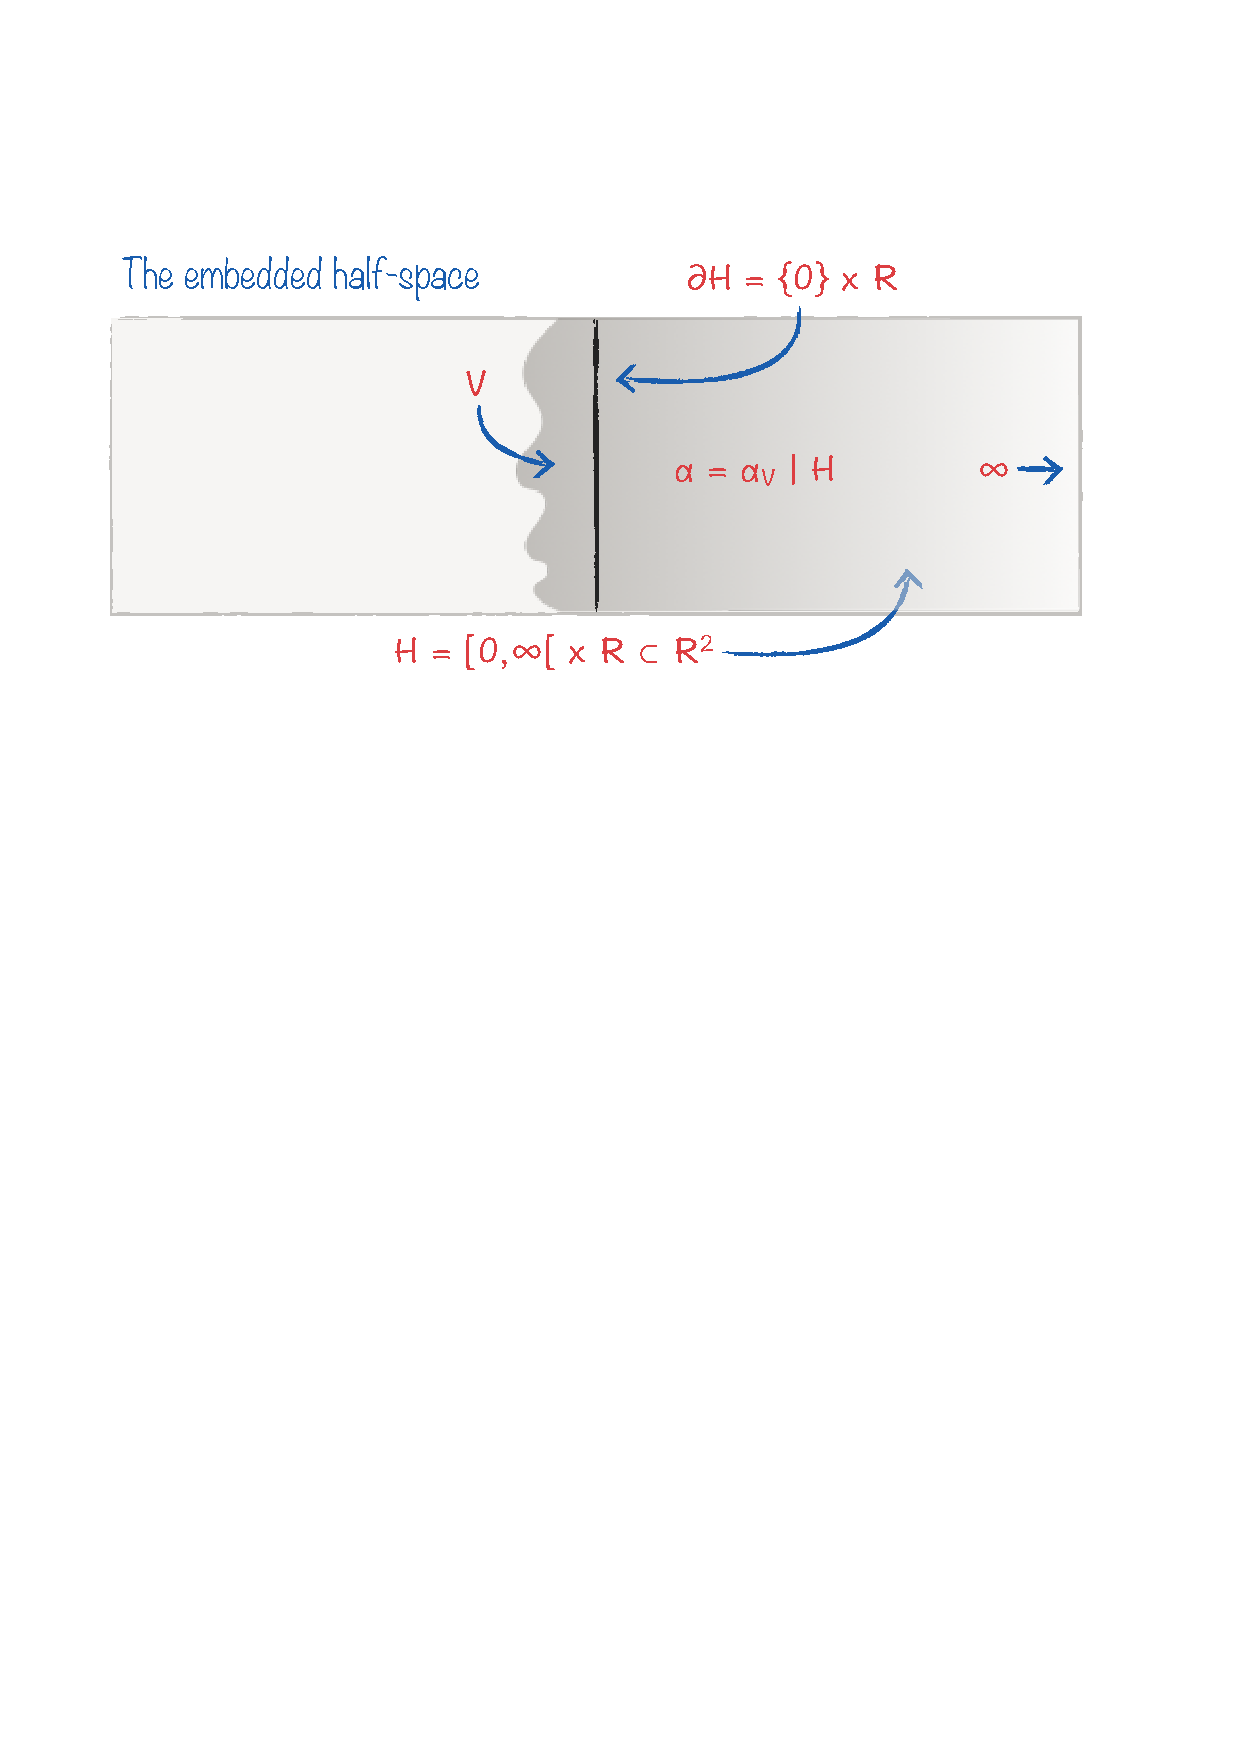
\includegraphics[width=\textwidth]{Figures/Half-space.jpg}}
